\documentclass[a4paper,11pt,fleqn,dvipsnames,oneside,openright,oldfontcommands]{memoir} 	% Openright aabner kapitler paa hoejresider (openany begge)

\usepackage{xfrac}
\usepackage{booktabs}
\usepackage[table,xcdraw]{xcolor}

%%%%%%%%% Indsat random
%makes it possible to refer to the name of a chapter rather than just the number.
\usepackage{nameref}
\usepackage{pdfpages}
\usepackage{marvosym}
\usepackage{setspace}
\usepackage{graphicx} % For at sætte 2 billeder ved siden af hinanden

%package for writing program code in latex
\usepackage{listings}
%%%%%%%%%%%%%%%%%%%%%%

% ¤¤ Oversaettelse og tegnsaetning ¤¤ %
\usepackage[T1]{fontenc}					% Output-indkodning af tegnsaet (T1)
\usepackage[danish]{babel}					% Dokumentets sprog
\usepackage[utf8]{inputenc}					% Input-indkodning af tegnsaet (UTF8)
\usepackage{ragged2e,anyfontsize}			% Justering af elementer
\usepackage{fixltx2e}						% Retter forskellige fejl i LaTeX-kernen			
\usepackage{gensymb}						% Nu kan der skrices procent tegn med \degree				
				
																							
% ¤¤ Figurer og tabeller (floats) ¤¤ %
\usepackage{graphicx} 						% Haandtering af eksterne billeder (JPG, PNG, EPS, PDF)
%\usepackage{eso-pic}						% Tilfoej billedekommandoer paa hver side
\usepackage{wrapfig}						% Indsaettelse af figurer omsvoebt af tekst. \begin{wrapfigure}{Placering}{Stoerrelse}
\usepackage{multirow}                		% Fletning af raekker og kolonner (\multicolumn og \multirow)
\usepackage{multicol}         	        	% Muliggoer output i spalter
\usepackage{rotating}						% Rotation af tekst med \begin{sideways}...\end{sideways}
\usepackage{colortbl} 						% Farver i tabeller (fx \columncolor og \rowcolor)
\usepackage{xcolor}							% Definer farver med \definecolor. Se mere: http://en.wikibooks.org/wiki/LaTeX/Colors
\usepackage{flafter}						% Soerger for at floats ikke optraeder i teksten foer deres reference
\let\newfloat\relax 						% Justering mellem float-pakken og memoir
\usepackage{float}							% Muliggoer eksakt placering af floats, f.eks. \begin{figure}[H]
\usepackage{array,booktabs,xcolor,longtable} % kan lave \hdashline i tabellertabe
\usepackage{arydshln}
\usepackage{tabu}
\usepackage{epstopdf} 						% Muligoer brugen af eps filer i latex

	
	
% ¤¤ Matematik mm. ¤¤
\usepackage{amsmath , amsthm , amsfonts , amssymb, float, stmaryrd} 		% Avancerede matematik-udvidelser
%\usepackage{mathtools}						% Andre matematik- og tegnudvidelser
\usepackage{textcomp}                 		% Symbol-udvidelser (f.eks. promille-tegn med \textperthousand )
\usepackage{rsphrase}						% Kemi-pakke til RS-saetninger, f.eks. \rsphrase{R1}
\usepackage[version=3]{mhchem} 				% Kemi-pakke til flot og let notation af formler, f.eks. \ce{Fe2O3}
\usepackage{siunitx}						% Flot og konsistent praesentation af tal og enheder med \si{enhed} og \SI{tal}{enhed}
\sisetup{output-decimal-marker = {,}}		% Opsaetning af \SI (DE for komma som decimalseparator) 

% ¤¤ Referencer og kilder ¤¤ %
\usepackage[danish]{varioref}				% Muliggoer bl.a. krydshenvisninger med sidetal (\vref)
\usepackage[numbers]{natbib}				% Udvidelse med naturvidenskabelige citationsmodeller
%%\usepackage[sort&compress,square,comma,numbers]{natbib}
\newcommand{\citer}[1]{\citeauthor{#1},~\citeyear{#1}~\cite{#1}}

%\DeclareRobustCommand{\citer}[1]{\citeauthor{#1},~\citeyear{#1}~\cite{#1}}
											% citere i teksten: "Et studie af 'forfatter', 'år' [kilde#] viser..."
%\usepackage{xr}							% Referencer til eksternt dokument med \externaldocument{<NAVN>}
%\usepackage{glossaries}					% Terminologi- eller symbolliste (se mere i Daleifs Latex-bog)
\usepackage{lastpage}					% Gør det mulig at refere til sidste side 

% ¤¤ Misc. ¤¤ %
\usepackage{listings}						% Placer kildekode i dokumentet med \begin{lstlisting}...\end{lstlisting}
\usepackage{lipsum}							% Dummy text \lipsum[..]
\usepackage[shortlabels]{enumitem}			% Muliggoer enkelt konfiguration af lister
\usepackage{pdfpages}						% Goer det muligt at inkludere pdf-dokumenter med kommandoen \includepdf[pages={x-y}]{fil.pdf}	
\pdfoptionpdfminorversion=6					% Muliggoer inkludering af pdf dokumenter, af version 1.6 og hoejere
\pretolerance=2500 							% Justering af afstand mellem ord (hoejt tal, mindre orddeling og mere luft mellem ord)


% Kommentarer og rettelser med \fxnote. Med 'final' i stedet for 'draft' udloeser hver note en error i den faerdige rapport.
\usepackage[footnote,final,danish,silent,nomargin]{fixme}		


%%%% CUSTOM SETTINGS %%%%

% ¤¤ Marginer ¤¤ %
\setlrmarginsandblock{3.0cm}{2.5cm}{*}		% \setlrmarginsandblock{Indbinding}{Kant}{Ratio}
\setulmarginsandblock{2.5cm}{3.0cm}{*}		% \setulmarginsandblock{Top}{Bund}{Ratio}
\checkandfixthelayout 						% Oversaetter vaerdier til brug for andre pakker

%	¤¤ Afsnitsformatering ¤¤ %
\setlength{\parindent}{0mm}           		% Stoerrelse af indryk
\setlength{\parskip}{3mm}          			% Afstand mellem afsnit ved brug af double Enter
\linespread{1,1}							% Linie afstand



% ¤¤ Indholdsfortegnelse ¤¤ %
\setsecnumdepth{subsection}		 			% Dybden af nummerede overkrifter (part/chapter/section/subsection)
\maxsecnumdepth{subsection}					% Dokumentklassens graense for nummereringsdybde
\settocdepth{section} 					% Dybden af indholdsfortegnelsen

% ¤¤ Lister ¤¤ %
\setlist{
  topsep=0pt,								% Vertikal afstand mellem tekst og listen
  itemsep=-1ex,								% Vertikal afstand mellem items
} 

%hyperlinks in the tabel of contents - comment this out before the report is printed.
\usepackage{hyperref}
\hypersetup{
	bookmarks = true,  % Show 'bookmark'-frame in pdf.
	colorlinks = true, % True = colored links, False = framed links.
	citecolor = black,  % Link color for references.
	linkcolor = black,  % Link color in table of contents.
	urlcolor = black,   % Link color for extern URLs.
}

% ¤¤ Opsaetning af figur- og tabeltekst ¤¤ %
\usepackage{caption}
\usepackage{subcaption}
\captionnamefont{\small\bfseries\itshape}	% Opsaetning af tekstdelen ('Figur' eller 'Tabel')
\captiontitlefont{\small}					% Opsaetning af nummerering
\captiondelim{. }							% Seperator mellem nummerering og figurtekst
\hangcaption								% Venstrejusterer flere-liniers figurtekst under hinanden
%\captionwidth{0.9\textwidth}					% Bredden af figurteksten
\setlength{\belowcaptionskip}{0pt}			% Afstand under figurteksten
\captionsetup[figure]{labelfont={bf,it},font={it}} % sætter nummer til fed og kursis. Resten til fed + skriften er mindre end resten
\captionsetup[table]{labelfont={bf,it},font={it}} 


% ¤¤ Opsaetning af listings ¤¤ %

\definecolor{commentGreen}{RGB}{34,139,24}
\definecolor{stringPurple}{RGB}{208,76,239}

\lstset{language=Matlab,					% Sprog
	basicstyle=\ttfamily\scriptsize,		% Opsaetning af teksten
	keywords={for,if,while,else,elseif,		% Noegleord at fremhaeve
			  end,break,return,case,
			  switch,function},
	keywordstyle=\color{blue},				% Opsaetning af noegleord
	commentstyle=\color{commentGreen},		% Opsaetning af kommentarer
	stringstyle=\color{stringPurple},		% Opsaetning af strenge
	showstringspaces=false,					% Mellemrum i strenge enten vist eller blanke
	numbers=left, numberstyle=\tiny,		% Linjenumre
	extendedchars=true, 					% Tillader specielle karakterer
	columns=flexible,						% Kolonnejustering
	breaklines, breakatwhitespace=true,		% Bryd lange linjer
}

% ¤¤ Navngivning ¤¤ %
\addto\captionsdanish{
	\renewcommand\appendixname{Appendiks}
	\renewcommand\contentsname{Indholdsfortegnelse}	
	\renewcommand\appendixpagename{Appendiks}
	\renewcommand\appendixtocname{Appendiks}
	\renewcommand\cftchaptername{\chaptername~}				% Skriver "Kapitel" foran kapitlerne i indholdsfortegnelsen
	\renewcommand\cftappendixname{\appendixname~}			% Skriver "Appendiks" foran appendiks i indholdsfortegnelsen
}

% ¤¤ Kapiteludssende ¤¤ %
\definecolor{numbercolor}{gray}{0.7}		% Definerer en farve til brug til kapiteludseende
\newif\ifchapternonum

\makechapterstyle{jenor}{					% Definerer kapiteludseende frem til ...
	\renewcommand\beforechapskip{0pt}
	\renewcommand\printchaptername{}
	\renewcommand\printchapternum{}
	\renewcommand\printchapternonum{\chapternonumtrue}
	\renewcommand\chaptitlefont{\fontfamily{pbk}\fontseries{db}\fontshape{n}\fontsize{20}{35}\selectfont\raggedright}
	\renewcommand\chapnumfont{\fontfamily{pbk}\fontseries{m}\fontshape{n}\fontsize{0.35in}{0in}\selectfont\color{black}}
	\renewcommand\printchaptertitle[1]{%
		\noindent
		\ifchapternonum
		\begin{tabularx}{\textwidth}{X}
			{\let\\\newline\chaptitlefont ##1\par} 
		\end{tabularx}
		\par\vskip-2.5mm\hrule
		\else
		\begin{tabularx}{\textwidth}{Xl}
			{\parbox[b]{\linewidth}{\chaptitlefont ##1}} & \raisebox{-5pt}{\chapnumfont \thechapter}
		\end{tabularx}
		\par\vskip2mm\hrule
		\fi
	}
}											% ... her

\chapterstyle{jenor}						% Valg af kapiteludseende - Google 'memoir chapter styles' for alternativer

% ¤¤ Sidehoved ¤¤ %

\makepagestyle{AAU}							% Definerer sidehoved og sidefod udseende frem til ...
\makepsmarks{AAU}{%
	\createmark{chapter}{left}{shownumber}{}{. \ }
	\createmark{section}{right}{shownumber}{}{. \ }
	\createplainmark{toc}{both}{\contentsname}
	\createplainmark{lof}{both}{\listfigurename}
	\createplainmark{lot}{both}{\listtablename}
	\createplainmark{bib}{both}{\bibname}
	\createplainmark{index}{both}{\indexname}
	\createplainmark{glossary}{both}{\glossaryname}
}
\nouppercaseheads											% Ingen Caps oenskes

\makeevenhead{AAU}{Gruppe 5406}{}{\leftmark}				% Definerer lige siders sidehoved (\makeevenhead{Navn}{Venstre}{Center}{Hoejre})
\makeoddhead{AAU}{\rightmark}{}{Aalborg Universitet}		% Definerer ulige siders sidehoved (\makeoddhead{Navn}{Venstre}{Center}{Hoejre})
\makeevenfoot{AAU}{\thepage}{}{}							% Definerer lige siders sidefod (\makeevenfoot{Navn}{Venstre}{Center}{Hoejre})
\makeoddfoot{AAU}{}{}{\thepage}								% Definerer ulige siders sidefod (\makeoddfoot{Navn}{Venstre}{Center}{Hoejre})
\makeheadrule{AAU}{\textwidth}{0.5pt}						% Tilfoejer en streg under sidehovedets indhold
\makefootrule{AAU}{\textwidth}{0.5pt}{1mm}					% Tilfoejer en streg under sidefodens indhold

\copypagestyle{AAUchap}{AAU}								% Sidehoved for kapitelsider defineres som standardsider, men med blank sidehoved
\makeoddhead{AAUchap}{}{}{}
\makeevenhead{AAUchap}{}{}{}
\makeheadrule{AAUchap}{\textwidth}{0pt}
\aliaspagestyle{chapter}{AAUchap}							% Den ny style vaelges til at gaelde for chapters
% ... her

\pagestyle{AAU}												% Valg af sidehoved og sidefod


%%%% CUSTOM COMMANDS %%%%

% ¤¤ Billede hack ¤¤ %
\newcommand{\figur}[4]{
		\begin{figure}[H] \centering
			\includegraphics[width=#1\textwidth]{billeder/#2}
			\caption{#3}\label{#4}
		\end{figure} 
}

% ¤¤ Specielle tegn ¤¤ %
\newcommand{\decC}{^{\circ}\text{C}}
\newcommand{\dec}{^{\circ}}
\newcommand{\m}{\cdot}


%%%% ORDDELING %%%%

\hyphenation{}

%%%%Fra engelsk til dansk i \autoref{•} %%%%
\renewcommand{\figureautorefname}{Figur}
\renewcommand{\sectionautorefname}{Afsnit}
\renewcommand{\subsectionautorefname}{Afsnit}
\renewcommand{\subsubsectionautorefname}{Afsnit}
\renewcommand{\tableautorefname}{Tabel}
\renewcommand{\appendixautorefname}{Appendiks}
\renewcommand{\equationautorefname}{Ligning}
\renewcommand{\itemautorefname}{Punkt}
\renewcommand{\chapterautorefname}{Kapitel}
\raggedbottom
%Figure references:
\newcommand{\figref}[1]{figur~\ref{#1}}

%Figure references after full stop/period:
\newcommand{\Figref}[1]{Figur~\ref{#1}}

%Table references:
\newcommand{\tabref}[1]{tabel~\ref{#1}}

%Table references after full stop/period:
\newcommand{\Tabref}[1]{Tabel~\ref{#1}}

%Appendix references:
\newcommand{\appref}[1]{appendiks~\ref{#1}}

%Appendix references after full stop/period:
\newcommand{\Appref}[1]{Appendiks~\ref{#1}}

%Section references:
\newcommand{\secref}[1]{afsnit~\ref{#1}}

%Section references:
\newcommand{\Secref}[1]{Afsnit~\ref{#1}}

%chapter references: 
\newcommand{\chapref}[1]{kapitel~\ref{#1}}

%chapter references: 
\newcommand{\Chapref}[1]{Kapitel~\ref{#1}}


%Units:
%inserting '\omit' before '{\put' prior ot final compile will fix allignment (and generate errors)
\newcommand{\unit}[1]{{\put(300,0){$\hfill\left[\: #1 \:\right]$}}}

%Text:
\newcommand{\tx}[1]{\text{#1}}

%Equation references:
%1 equation:
\renewcommand{\eqref}[1]{ligning~(\ref{#1})}
%2 equations:
\newcommand{\eqrefTwo}[2]{ligning~(\ref{#1}) og (\ref{#2})}
%3 equations:
\newcommand{\eqrefThree}[3]{ligning~(\ref{#1}), (\ref{#2}) og (\ref{#3})}
%4 equations:
\newcommand{\eqrefFour}[4]{ligning (\ref{#1}), (\ref{#2}), (\ref{#3}) og (\ref{#4})}
%5 equations:
\newcommand{\eqrefFive}[5]{ligning (\ref{#1}), (\ref{#2}), (\ref{#3}), (\ref{#4}) og (\ref{#5})}


%Equation references after full stop/period:
%1 equation:
\newcommand{\Eqref}[1]{Ligning~(\ref{#1})}
%2 equations:
\newcommand{\EqrefTwo}[2]{Ligning~(\ref{#1}) og (\ref{#2})}
%3 equations:
\newcommand{\EqrefThree}[3]{Ligning~(\ref{#1}), (\ref{#2}) og (\ref{#3})}
%4 equations:
\newcommand{\EqrefFour}[4]{Ligning (\ref{#1}), (\ref{#2}), (\ref{#3}) og (\ref{#4})}
%5 equations:
\newcommand{\EqrefFive}[5]{Ligning (\ref{#1}), (\ref{#2}), (\ref{#3}), (\ref{#4}) og (\ref{#5})}
\begin{document}
\frontmatter
\clearpage
\thispagestyle{empty}

%\begin{figure}[H]
%	\raggedleft
%		
\includegraphics[width=0.2\textwidth]{figures/aaulogo-da.png}
%\end{figure}


%\vspace*{\fill} 
%\begin{center}	
%	\begin{Huge}
%		P3 Projektrapport - efterår 2015\\
%		\vspace{5 mm}
%		\textbf{System til detektering af kropsbalance}\\
%		\vspace{3 mm}
%		Gruppe 375
%	\end{Huge}
%\end{center}
%\vspace*{\fill}

\begin{center}
	\vspace*{\baselineskip}
	\rule{\textwidth}{1.6pt}\vspace*{-\baselineskip}\vspace*{2pt} % Thick horizontal line
	\rule{\textwidth}{0.4pt}\\[\baselineskip] % Thin horizontal line
	
	{\huge Aktivitetsmåler til forebyggelse\\\hspace*{2ex} af fysisk inaktivitet hos børn \\[0.5\baselineskip] \large Projektrapport 4. semester}\\[0.2\baselineskip] % Title
	
	\rule{\textwidth}{0.4pt}\vspace*{-\baselineskip}\vspace{3.2pt} % Thin horizontal line
	\rule{\textwidth}{1.6pt}\\[\baselineskip] % Thick horizontal line
	\vspace*{5\baselineskip}
	\begin{figure}[H]
		\centering
		\begin{minipage}[c]{1\textwidth}
			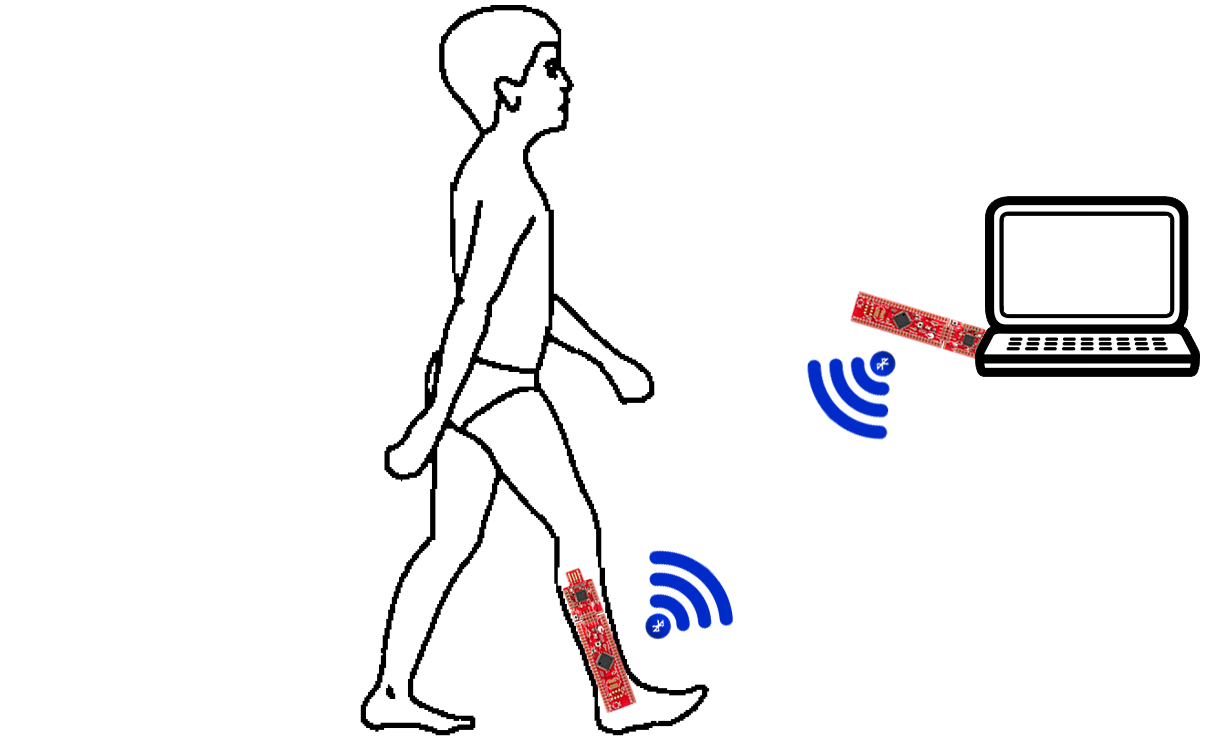
\includegraphics[width=.75\textwidth]{figures/forside2.PNG}
		\end{minipage}
		\hfill
	\end{figure}
	\vspace*{\fill}
	\scshape % Small caps
	{\Large Gruppe 4403\par}
	
	\vspace*{.8\baselineskip} % Whitespace between location/year and editors
	
	Aalborg Universitet,  01/02/2016 - 27/05/2016 \par % Location and year
\end{center} % Center all text
%{\color{white}X \\ X \\ X \\}

%\begin{center}
%	\textit{Gruppemedlemmer:}\\
%	Cecilie Sophie Rosenkrantz Topp, Frederik Skou Nielsen \\
%	Josefine Dam Gade, Line Sofie Hald, Morten Skaarup Larsen
%\end{center}
\begin{center}
	\line(1,0){400}
\end{center} \clearpage
\mainmatter
\chapter{Introduktion}\vspace{-0.75cm}
% baggrund for projektet
Artrose er den mest udbredte gigtsygdom og en af de mest udbredte kroniske sygdomme i Danmark. 
%(\textbf{Note: tilføj hvad en kronisk sygdom er}) \citep{sygdom}. 
Artrose er en kronisk ledsygdom der kan ramme alle ledstrukturer, men primært rammes ledfladernes bruskdele \citep{schroder}. Prævalensen for artrose i Danmark er omkring 800.000 personer, og der sker årligt over 20.000 indlæggelser med artrose som aktionsdiagnose. \citep{sygdom}
Forekomsten af artrose stiger med alderen, hvor personer over 55 år repræsenterer den største gruppe af artrosepatienter. Over de seneste 15 år er der sket en stigning i antallet af knæalloplastikker fra 2.500 i år 2000, til 9.800 i år 2015. \citep{aarsrapport2016} \\
Knæet er det led hvor artrose  hyppigst forekommer. Knæartrose er den førende årsag til funktionsnedsættelse i de nedre ekstremiteter \citep{bezwick2012}. 
Ved knæartrose nedbrydes nedbrusken, hvilket medfører at der forløber en række reaktioner i knoglen under brusken, samt i synovialmembranen \citep{brostrom2012}. Som følge af nedbrydning af brusk kan der opstå ledskurren og fejlsstilling, hvilket kan medføre belastningssmerter og i sidste ende funktionstab \citep{ugeskrift2011}.
Der er stor variation i hvordan personer der lever med knæartrose påvirkes, og nogle vil derfor kunne leve relativt upåvirkede med sygdommen, mens andre vil opleve at sygdommen svækker både arbejdsevne og livskvalitet \citep{sygdom}. Knæartosepatienter kommer igennem et længere behandlingsforløb, men da knæartrose er irreversibel, kan artrose kun afhjælpes og ikke kureres, og de fleste ender med at få en total knæalloplastik (TKA). \citep{brostrom2012} \\ 
% intro til projektet
Ifølge sundhedsstyrelsens vurdering er knæalloplastik effektiv til at mindske smerte, øge funktion og derved forbedre livskvalitet, og idet TKA-operationen er den sidste behandlingsmulighed, er patientens operationstilfredshed en betydningsfuld faktor. %det vigtigt at opnå dette mål. Det ses dog hos TKA-patienter at 19\% efter den primære operation og 47\% efter revision fortsat oplever svære smerter \citep{Petersen2015}. 
Et studie af \citer{Bourne2010} viser imidlertid, at 11 til 25\% af TKA-patienter er utilfredse efter operationen, hvorved behandlingen fra et patientøjemed ikke vurderes som succesfuldt.
Modsat ses det af sundhedsstyrelsens årsrapport for TKA-perationer, at alle succeskriterier overholdes for størstedelen af operationer. \citep{aarsrapport2016} 
Der opstår således et dilemma i TKA-behandling af knæartrose, set fra sygehusvæsenets perspektiv, er succesfuldt, men fra 11-25\% af patienternes synspunkt er utilfredsstillende.

\section*{Initierende problemstilling}
\begin{center}
	\textit{Hvorfor får nogle knæartrose patienter kroniske postoperative smerter efter en total knæalloplastik?}
\end{center}


\chapter{Problemanalyse - udsnit}\vspace{-.75cm}
\textit{Følgende afsnit blot uddrag af problemanalysen og dermed er al indhold ikke vedhæftet.}
\section{Knæartrosepatienters forløb}
En længere række faktorer har betydning for udviklingen af knæartrose. Hvis en eller flere af disse faktorer er tilstede, er den påvirkede mere disponeret for knæartrose. Dette sker ved overbelastning igennem arbejde og fritid, tidligere knæskader, genetisk arv, overvægt samt køn \citep{brostrom2012}. Knæartrose er til stede blandt 45\% af alle over 80 år. Antallet af personer med knæartose kan formodes at stige da levealderen i Danmark stiger. %Dette er ikke den eneste faktor, hvorfor prævalensen kan antages at stige. 
En anden risikofaktor for udviklingen af knæartrose er overvægt. Ydermere stiger andelen af overvægtige med alderen, hvilket ligeledes er tilfældet for knæartrose. \citep{Vestergaard2014} \citep{Vestergaard2016} \citep{Lind2016} \citep{Lind2016b} 
%Overvægtige med en høj body-mass-index (BMI>30\citep{definitionfedme1999}) er disponeret for knæartrose med en relativ risiko på en faktor tre, hvoraf en kombination af ovenstående faktorer øger risikoen for lidelsen. Dog kan der opstå problematikker vedrørende benyttelsen af BMI, da metoden ikke skelner mellem fedt og muskler. \textbf{(8)} \citep{brostrom2012} \citep{Vestergaard2014} \citep{Vestergaard2016} \citep{Lind2016} \citep{Lind2016b}

En patients symptomer kan medføre igangsættelsen af et behandlingsforløb. Et behandlingsforløb for en patient med knæartrose består af flere faser, hvis mål er smertelindring, mobilitetsforøgelse samt forebyggelse. Generelt kan faserne opdeles i non-invasive og invasive behandlingsmetoder. Hvilken behandlingsmetode som hjælper patienten afhænger af graden af knæartrose. \citep{Lind2016b}

\begin{figure}[H]
	\centering
	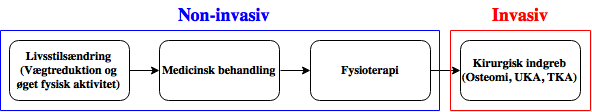
\includegraphics[width=0.9\textwidth]{../figures/bProblemanalyse/flowchart_behandlingsforloeb.png}
	\caption{På figuren ses et flowchart indeholdende de forskellige behandlingsmetoder der forekommer igennem et patientforløb med knæartrose.}
	\label{fig:flow_behandlingsfaser}
\end{figure}\vspace{-.25cm}

Patientgruppen som postoperativt er utilfredse er svært definerbar. Problematikken opstår i og med klassificeringen bag de potentielt 11 til 25~\% utilfredse patienter er vedrørende postoperative smerte samt funktion. Flere studier indikerer at de utilfredse patienter har signifikant flere smerte og signifikant større funktionsnedsættelse, end de tilfredse patienter \citep{Bourne2010} \citep{Jacobs2014}. Det kan forestilles at der blandt nogle af patienterne findes en forventningsfaktor, hvilket gør de postoperativt kategoriserer sig selv som værende utilfreds, omend de har opnået en forbedring af både smerte og/eller mobilitet.

%Det kan tænkes at forventningsfaktoren kan være medvirkende til at kategorisere dem som værende utilfredse, som resultat af skuffelsen af ikke at fungere som et individ med et fuldt funktionsdygtigt knæ. Denne antagelse understøttes af \citer{Bourne2010}, som beskriver de største prædiktorer omhandlende utilfredshed efterfulgt af en TKA-operation. Den faktor som besidder den største score er, patientens forventninger til operationen ikke er mødt, hvilket medfører 10,7 gange større risiko for utilfredshed. \citep{Bourne2010} 
%I et andet studie af \cite{Keudell2013} bliver patienternes alder sammenkoblet med deres forventninger. Det tyder på at den ældre patientgruppe (>65 år) har generelt har lavere forventninger til operationsresultatet, end den yngre patientgruppe (<55 år). I dette studie indikeres det at den ældre patientgruppe generelt har større tilfredshed, end den yngre. Dette kan antages at have en sammenhæng med påstanden fra \cite{Bourne2010}, vedrørende prædiktoren til utilfredshed, omhandlende forventninger til operationen. \textbf{NOTE:(7 (mangler analyse?))}

\section{Kirurgisk behandling}
Knæalloplastik er et operativt indgreb der har til formål helt eller delvist at udskifte knæleddet, med specielt designede metal- og plastkomponenter som varig erstatning for bruskfladerne i knæet. Operationen opdeles i TKA og UKA, hvilket henholdsvis er helt eller delvis udskiftning af knæleddet og afhænger af den specifikke diagnose. Der kan ved traume tilfælde eller svære beskadigelser af de anatomiske strukturer omkring knæet forekomme specialiserede udgaver af knæalloplastik.

\begin{figure}[H] 
	\begin{center}
		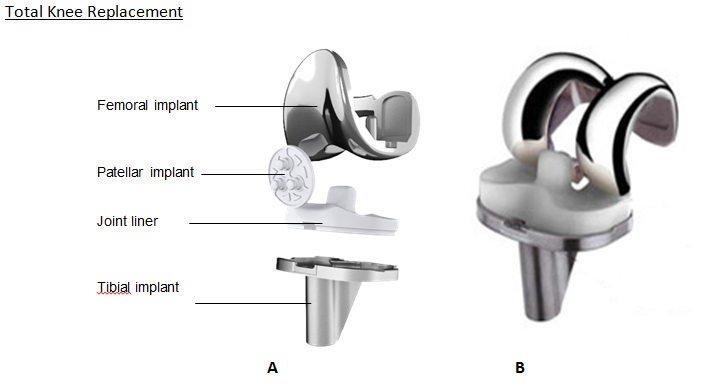
\includegraphics[width=0.55\textwidth]{../figures/tka_implant}
	\end{center}
	\caption{Komponenterne til en total knæalloplastik, består af et femural og tibial implantat ofte bestående af en titaniumlegering. Patella- og tibiaindsatsen er lavet af polyethylen, hvilket er med til at mindske friktionen og efterligne knæledes naturlige bevægelse. \citep{robodoc2016}} 
	\label{fig:tka_implant} 
\end{figure} \vspace{-.50cm}

Efter en vellykket operation burde patienterne ikke på længere sigt ikke opleve smerter, dette er imidlertid ikke tilfældet.

Efter en vellykket operation burde patienterne på længere sigt ikke opleve smerter, dette er imidlertid ikke altid tilfældet. Der er således et problem med resultatet af operationen, på trods af operationen overholder sundhedsstyrelsens succeskriterier \citep{aarsrapport2016}. 

\section{Smerte}
Smerte er af The International Association for the Study of Pain (IASP) defineret som: “\textit{An unpleasant sensory and emotional experience associated with actual or potential tissue damage, or described in terms of such damage.}” \citep{Carmon}.
%Smerter registreres af noiceptorer i kroppen. De fleste smertereceptorer er frie neuronender som forgrener sig ud i hele kroppen, og ligger frit i væv. De dækker således et stort område og kan reagere på forskellige typer stimuli som vævet bliver udsat for. Typen af stimuli bliver bestemt afhængig af hvilke nociceptorer som aktiveres. Forskellige nociceptorer besidder forskellige typer af natrium-/kaliumporte, som aktiveres ved temperaturændring, trykforandring og kemisk foranding, som ses på figur \ref{neuronport}.
Der findes flere måder at opdele og kategorisere smerte på, men generelt kan det opdeles i to overordnede kategorier; akut og kronisk. Efter TKA-operationer oplever patienter akut smerte, men denne fortager sig hurtigt hvis alt forløber som forventet. Problemet opstår når patienterne får kroniske postoperative smerter. Kronisk smerte er af IASP defineret som at være smerteperception som varer længere end det generelt ville forventes. Oftest sættes denne grænse ved tre måneder \citep{Carmon}. Kronisk smerte kan skyldes fejltilstande i nervesystemet på baggrund af akutte nociceptiske eller neuropatiske skader. Efter den akutte smerte har fortages sig, fortsætter smerteperceptionen, tilsyneladende uden grund. Patienten kan så opleve konstant smerte, periodisk smerte, smerte ved bevægelse eller opbyggende smerter. \citep{Giangregorio1997} Da smerterne ikke opstår som følge af operative fejl kan det antages at nogle patienter allerede før operationen er disponeret til at få kroniske postoperative smerter. Herfor er det relevant at undersøge hvilke metoder der anvendes til udvælgelse af patienter.
%Kronisk smerte kan også være af psykogen oprindelse. Psykogene smerter er en imaginær perception af smerte, og derved besværlig at præcisere, idet der ikke er og muligvis aldrig har været en fysisk årsag til smerten. Hos en person med psykogene smerter er hjernen fuldt overbevidst om, at den oplever fysiske, nociceptiske eller neuropatiske, smerter og lider deraf. Smerten er udelukkende psykisk hos personen, men er af den grund ikke mindre virkelig, grundet smertes subjektive natur. \citep{Giangregorio1997}

\section{Klinisk udvælgelse af patienter til TKA-operation}
%Patienter som tilbydes en TKA udvælges på baggrund af en læge eller kirurgs observationer og erfaringer.
Sundhedsstyrelsen har udarbejdet nationale retningslinjer for hvordan udvælgelsen til TKA-operation skal ske. Udvælgelsen udføres af en læge eller kirurg, ved hjælp af retningslinjerne og dennes personlige observationer og erfaringer. Patienter kan hermed opleve forskellige anbefalinger og behandlingsmuligheder ved forskellige klinikere. \citep{brostrom2012} \\
%Sundhedsstyrrelsen har udarbejdet nationale retningslinjer samt en række indikationer som kan få klinikeren til at fravælge en patient til en operation. Disse indikationer er eksempelvis infektioner i knogler eller leddet, hvis patienten ingen smerter har i leddet eller hvis patienten har en kort forventet levetid. 
%En anden indikator, som kan få en kliniker til at fravælge at operere patienten, er hvis patienten har urealistiske forventninger til operationen.
Et studie af \citer{skou2016} har fundet en uoverenstemmelse mellem hvilke faktorer kirurgere fandt vigtigst for patientens egnethed til TKA og hvilke faktorer de samme kirurger udvalgte patienter ud fra. Denne uoverensstemmelse viser hvor kompleks udvælgelsesprocessen til en TKA-operation er, samt vanskelighederne ved at bestemme hvilke faktorer der har størst betydning for en klinikers beslutningsprocess. Udfra resultaterne fra studiet af \citer{skou2016} antydes det at klinikerne anvender både bevidste og ubevidste faktorer til bestemmelse af patienters egnethed til en TKA. Desuden er det fundet at klinikerne har svært ved at vurdere patienter, hvis ikke der er klare indikationer som gør patienten enten egnet eller uegnet til en TKA-operation. 
I de tilfælde hvor der ikke er klare indikationer på at patienten vil have gavn af en TKA, vil en teknologisk metode der kan hjælpe klinikeren med at vurdere patienten være fordelagtig. Teknologien skal bidrage til beslutningen, og ekskludere patienter fra operationen som har større risiko for udvikling af kroniske smerter.

\section{Teknologier til vurdering af smerte}
For at understøtte klinikerens vurdering af de enkelte patienter vedrørende henstilling til en TKA-operation, kan det overvejes, hvorvidt det vil være hensigtsmæssigt at tilføje en ekstra undersøgelse til patientens behandlingsforløb forud for beslutningstagen. %Relevante undersøgelser indebære objektive målinger af neural aktivitet i forskellige situationer, samt vurdering af patienternes individuelle respons på forskellige typer af stimuli. 
Der findes flere teknologier som objektivt vil kunne undersøge patienters perception af smerte og reaktion på stimuli, men der fokuseres i tilsendte materiale udelukkende på quantitative sensory testing (QST). \\
QST er en metode til objektiv undersøgelse af det sensoriske nervesystems funktion. %Metoden kan anvendes til undersøgelse af forskellige egenskaber, herunder smertegrænser. 
Metoden eksponerer patienten for forskellig sensorisk sensation, som varme, kulde, vibration og tryk. Patienten placerer sin opfattelse af smerten på en VAS (Visual Analog Scale) hvor smerten rangeres mellem 1 (mindst smerte) til 10 (værst tænkelige smerte). Dermed er det muligt at identificere patientens perception af smerte.
QST bliver i forskningsregi anvendt til undersøgelse af patienter der får udført en TKA-operation. I et studie af \citer{Martinez2007} undersøges 20 patienter med artrose i knæet før og efter TKA-operation. Formålet hermed var at identificere faktorer, der har indvirkning på udviklingen af postoperative smerter. 
%%QST blev udført henholdsvis før operationen og efterfølgende en og fire dage samt en og fire måneder efter operationen. Parametrene der blev undersøgt i QST'en var tærskelværdier for temperatur, mekanisk smerte og hvordan de enkelte patienter responderede på en eksponering for temperaturer over tærskelværdierne. 
Studiet fandt, at der forekommer en sammenhæng mellem periodiske smerter efter operationen og de patienter, der oplever hyperalgesi (øget smertesensitivitet) under eksponering for varme præoperativt. \citep{Martinez2007} 
%Der skal imidlertid tages højde for, at der er flere fejlkilder forbundet med QST, da nøjagtigheden i høj grad afhænger af både patientens og undersøgerens præcision under udførelsen af de enkelte tests. Det må således forventes, at der kan forekomme variationer mellem enkelte QST udført på den samme patient. \citep{Yarnitsky2006}

\section{Problemafgrænsning}
Selvom TKA-operationerne bliver udført overholder succeskriterierne, er 11 til 25\% af patienterne stadig utilfredse. Det tyder på at disse patienter er utilfredse på grund af deres manglende resultater efter operationen, relateret til smerte og funktionsnedsættelse. Klinikerne er ansvarlig for belsutningstagen hvorvidt en patient er egnet til at modtage en TKA-operation. Klinikerne formår succesfuldt at udvælge 75 til 81\% af patienterne, på baggrund af deres erfaring, radiologiske fund, symptom vurdering, samt patientens egne udtalelser. Den resterende patientgruppe er utilfredse med resultatet, hvilket indikerer at udvælgelsesmetoden ikke er god nok, og at eventuelle bias kan have medvirket til dette resultat. Det kunne derfor, for klinikeren og patienten være fordelagtigt hvis den benyttede metode blev forbedret. Forbedringen kan indebære benyttelse af en teknologisk metodik. Den teknologiske tilgang skulle medføre nogle faktiske resultater som skal supplere og bidrage til klinikerens beslutningstagen. Hvis en teknologisk metode skal kunne implementeres kræves det at denne muliggør identificering af patientgruppen, hvis risiko for udviklingen af kroniske postoperative smerter, er størst. Den teknologiske tilgang bør ydermere være minimalt invasiv og omkostningseffektiv. Disse kriterier opfyldes på bedst af QST, blandt de analyserede smerteklassificeringsmetoder, hvormed det antydes at QST vil være den teknologiske tilgang som bedst vil kunne supplere klinikerens beslutningstagen. 
\subsection*{Problemformulering}
\begin{center}
	\textit{Hvilke konsekvenser er der forbundet med en implementering af QST som supplement til klinikerens vurdering af patienten til indstilling til TKA, på de ortopædkirurgiske afdelinger i Region Nordjylland?}
\end{center}

\chapter{Fremtidig metode}\vspace{-.75cm}
Til besvarelse af problemformuleringen anvendes Health Technology Assessment core (HTA-core) modellen. Målet med HTA-core modellen er at analysere og diskutere de essentielle problemstillinger ved en given teknologi, samt at præsentere resultaterne fundet ved analysen og diskussionen \citep{HTAcore}. Ydermere bidrager benyttelsen af HTA-core modellen til en systematisk og bred vurdering af den givne teknologi. Dette bidrager til at grundlag for at træffe beslutninger på baggrund af evidens. \citep{mtvhaandbog2007} \citep{HTAcore}  HTA-core modellen kan anvendes til besvarelse af problemformuleringen, da problemformuleringen lægger op til en analyse af problemstillinger ved QST set ud fra et sundhedsvidenskabeligt perspektiv. Ved anvendelse af HTA-core inddeles analysen af teknologien i følgende ni forskellige områder. \citep{HTAcore}

\begin{enumerate}
	\item Sundhedsmæssigt problem og nuværende brug af teknologien (CUR)
	\item Beskrivelse og tekniske karakteristika for teknologien (TEC)
	\item Sikkerhed (SAF)
	\item Klinisk effektivitet (EFF)
	\item Omkostninger og økonomisk evaluering (ECO)
	\item Etisk analyse (ETH)
	\item Organisatoriske aspekter (ORG)
	\item Patient- og sociale aspekter (SOC)
	\item Juridiske aspekter (LEG)
\end{enumerate}

Hver af disse områder belyser bestemte problemstillinger ved implementering af teknologien. For yderligere at præcisere hvilke vinkler indenfor hvert område der er relevante at undersøge med hensyn til implementeringen af QST som supplement til klinikerens belsutningstagen, opdeles områderne i emner og problematikker. Tilsammen udgør område, emner og problematikker et vurderingselement, som er relevant for besvarelsen af problemformuleringen.

\begin{figure}[H] 
	\begin{center}
		\includegraphics[width=0.5\textwidth]{../figures/cMetode/vurderingselement}
	\end{center}
	\caption{Figuren viser, hvordan vurderingselementet samlet er udgjort af de tre elementer; område, emner og problematikker.} 
	\label{fig:vurderingselement} 
\end{figure} \vspace{-.50cm}

Ikke alle vurderingselementer i HTA-core er relevante, til vurdering af alle typer af teknologier. Ved eksklusion  af et vurderingselement argumenteres der for hvorfor dette element ikke er relevant i den pågældende HTA. \citep{HTAcore} Eksempelvis er det i dette projekt valgt ikke at inkludere det første område “Sundhedsmæssigt problem og nuværende brug af teknologien”, da emnerne og problematikkerne indenfor dette område besvares af problemanalysen, som blev lavet forud for problemformuleringen. Hermed vil en inkludering af dette område i HTA’en ikke føre til indsamling af ny viden, hvorfor det er valgt at ekskludere dette område. 

Til besvarelse af den opstillede problemformulering er hver af de tilbageværende otte områder uddybet med emner og problematikker. Eksempelvis er der under TEC området opstillet tre emner; teknologiens egenskaber, teknologiens begrænsninger og sammenligning med nuværende teknologier. Hver af disse emner er uddybet med en til fire problematikker. Før besvarelse af hver af disse problematikker argumenteres der for den enkelte problematiks relevans for besvarelsen af problemformuleringen, hvilket sikrer at, kun de problematikker der bidrager til  besvarelse af problemformuleringen besvares i projektet. Efter analyse af hvert område opsummeres vigtige pointer og resultater fra analysen i en delkonklusion. Disse delkonklusioner anvendes videre i syntesen til udarbejdelse af diskussion og konklusion for hele projektet.    

\chapter{Projektets tidsplan}
\begin{figure}[H] 
	\begin{center}
		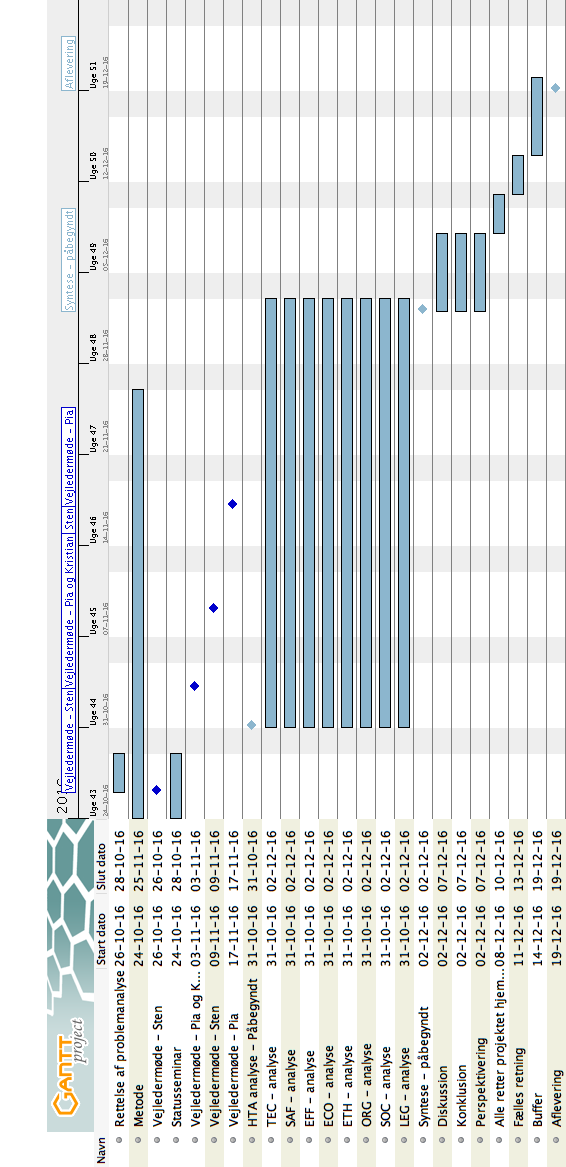
\includegraphics[width=0.6\textwidth]{../figures/cMetode/Projekt_tidsplan}
	\end{center}
%	\caption{} 
	\label{fig:tidsplan} 
\end{figure} \vspace{-.50cm}

\begingroup
\label{litteraturliste}
\raggedright
\bibliographystyle{unsrtnat}
\bibliography{../kilder}
\endgroup


\end{document}




